% !TEX encoding = UTF-8 Unicode
% !TEX root = thesis-ex.tex

This discussion is based on the model introduced in Ref.~\cite{Tachibana:2017syd}.
This model considers the evolution of the jet and QGP in a coupled manner, considering the energy and transverse momentum exchange between them.
In this picture, both the jet and medium are allowed to modify each other; the jet is modified via collisional and radiative processes while the medium evolves hydrodynamically and is modified because it picks up the energy lost by the jet.

The time evolution of the jet is given by a set of coupled transport equations that describe the energy and transverse momentum distributions of the partons within the jet. These are given as

\begin{gather}
f_i (\omega_i, \kTsq_i, t) = \frac{dN_i (\omega_i \kTsq_i, t)}{d \omega_i d\kTsq_i} \\
\nonumber \\
\frac{d f_j}{dt} = \hat{e_j} \frac{\p f_j}{\p \omega_j} + \frac{1}{4} \hat{q_j} \nabla_{\kT}^2 f_j 
 + \sum_i \int d\omega_i d\kTsq_i \frac{d\widetilde{\Gamma}_{i\rightarrow j} }{d\omega_j d\kTsq_j dt} f_i 
 - \sum_i \int d\omega_i d\kTsq_i \frac{d\widetilde{\Gamma}_{j\rightarrow i} }{d\omega_ij d\kTsq_i dt} f_i
\label{eq:jf_transportEq} 
\end{gather}
where $i$ is the type of parton, $\omega_i$ is its energy, and $\kTsq$ is its transverse momentum with respect to the jet axis.
The first term in Equation~\ref{eq:jf_transportEq} is the collisional energy loss, the second term is the transverse momentum broadening, and the last two terms are the medium induced gain and loss radiative processes respectively.
The splitting processes are are given by:

\begin{align}
\frac{d\Gamma_{i \rightarrow j}}{d \omega_j d\kTsq_j dt} = \frac{2\alpha_S}{\pi} \hat{q}_g \frac{x P_{i \rightarrow j} (x)}{\omega_j {k_{\rm T}^4}_j} \sin^2 \left(\dfrac{t - t_i}{2\tau_f} \right)
\end{align}
where $P_{i \rightarrow j} $ is the vacuum splitting function for $i \rightarrow j $ with $\omega_j$ being the energy of the radiated parton, $\tau_f$ is the formation time of the radiated parton, and $\kT_j$ is the transverse momentum of the radiated parton with respect to the parent parton.
These transport Equations~\ref{eq:jf_transportEq} can be solved numerically and agree with \RAA\ measurements \cite{Aad:2014bxa, Khachatryan:2016jfl, Abelev:2013kqa}.
The effects of the medium are included by considering the energy-momentum conservation of the jet-QGP system $ \p_\mu [T_{\rm QGP}^{\mu\nu} + T_{\rm jet}^{\mu\nu}] = 0$.
Then the source term $J^\nu(x)$ that describes the energy transfer between the jet and the medium can be defined as $J^\nu(x) \equiv -\p_\mu  T_{\rm jet}^{\mu\nu}$, making the QGP evolution being given by

\begin{align}
 \p_\mu T_{\rm QGP}^{\mu\nu} = j^\nu
\end{align}
which characterizes the energy-momentum transfer between the jet and the QGP.

An important component of this model is the flow induced by jets.
This can be seen in Figure~\ref{fig:jf_snapshot}, where the evolution of the energy density of the medium can be seen in a sample event.
A single jet travels through the QGP, and can be clearly seen in the lower panels after the energy of the medium has been subtracted out.
The ``V'' shaped feature seen is the mach cone that is induced by the parton as it moves faster than the medium sound velocity.


\begin{figure}[htbp]
\begin{center}
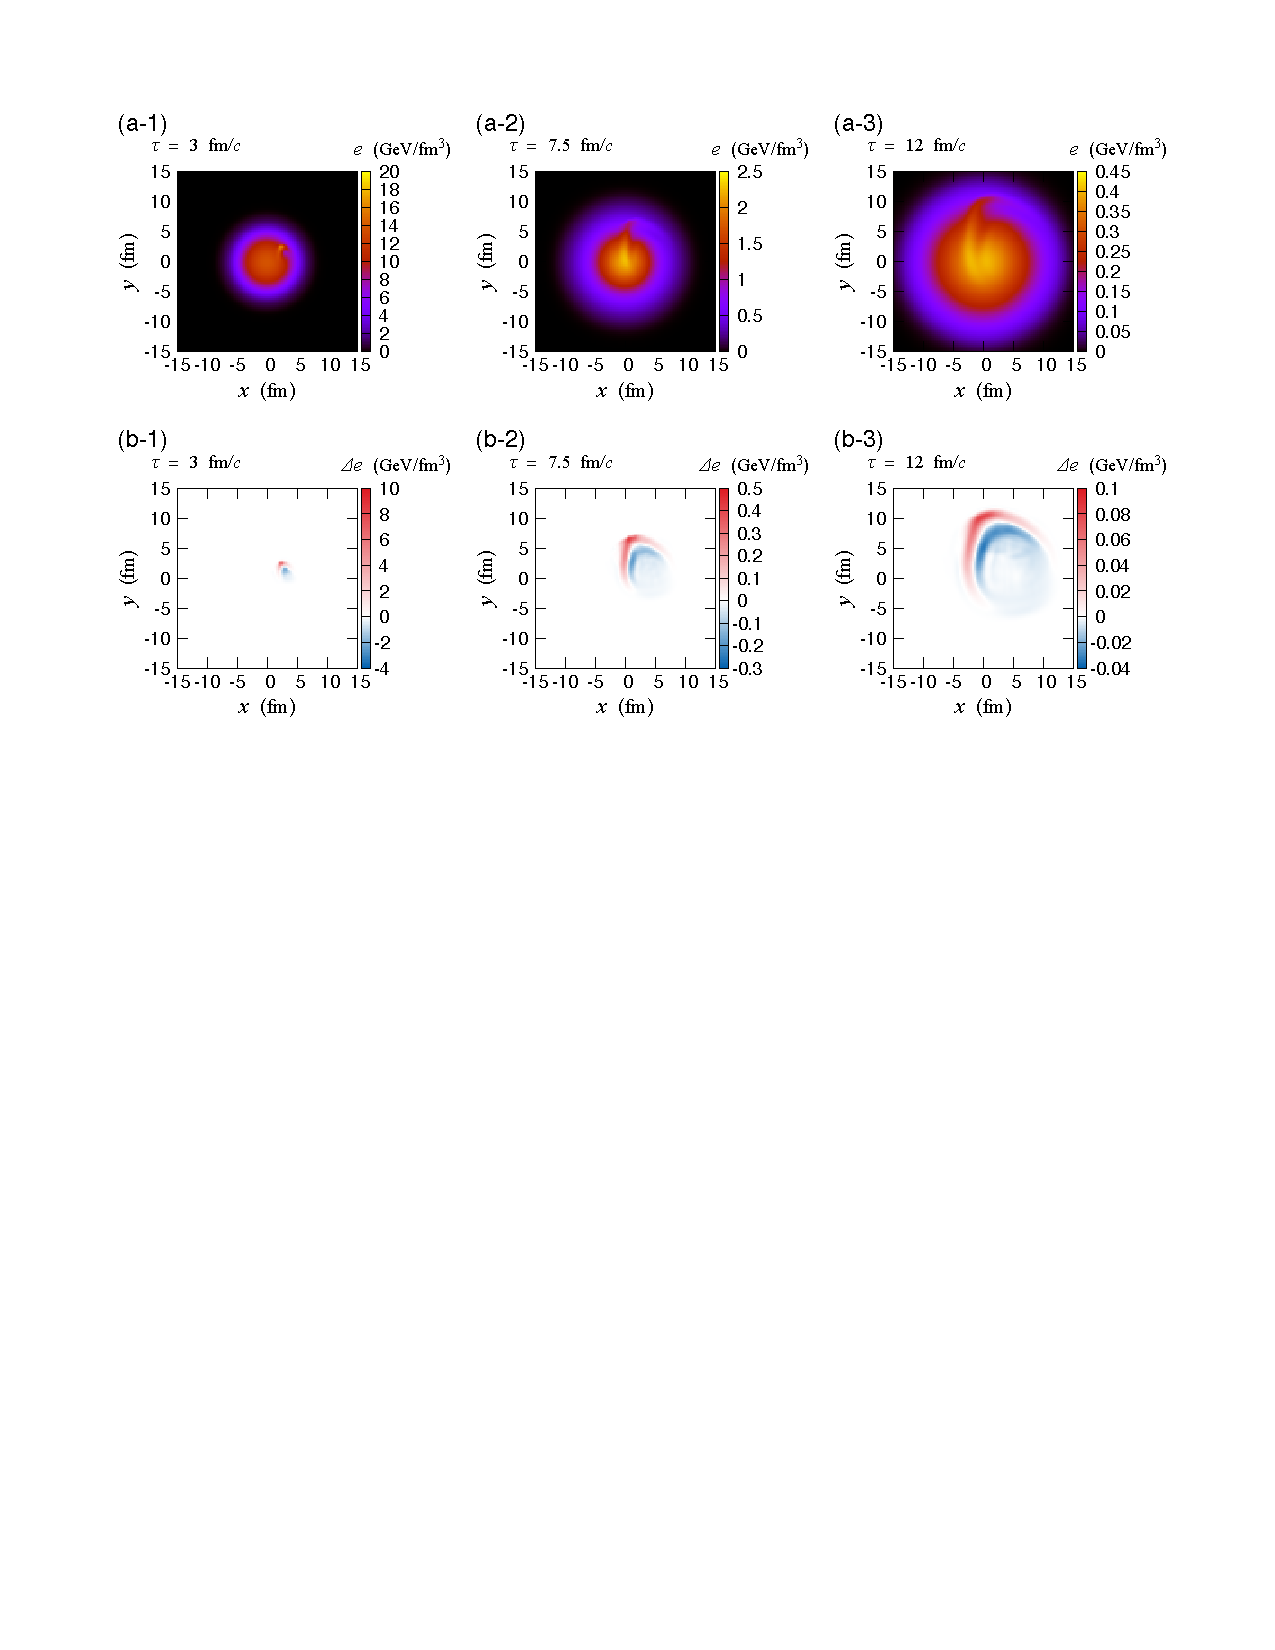
\includegraphics[width=0.85\textwidth]{figures/jetMeasurements/JF_snapshot}
\caption{(Top) The time evolution of the energy density of the quark gluon plasma with a jet propagating through it.
(Bottom) The time evolution of the energy density in the event after the energy density of the QGP has been subtracted out.
Figure from Ref.~\cite{Tachibana:2017syd}.}
\label{fig:jf_snapshot}
\end{center}
\end{figure}

The final jet energy has two components: the jet shower, and the hydrodynamic response.
The former as discussed above comprises of the collisional energy loss, momentum broadening, and medium induced radiation.
The latter includes the energy lost from the jet shower that thermalizes into the medium and induces conical flow, some of which is still in the jet cone.
This compensates some of the energy lost in the shower and can be seen in Figure~\ref{fig:jf_energyLoss}.
While the absolute amount of energy lost increases as a function of initial jet energy, the fractional energy loss decreases.
Furthermore there is a cone size dependence once the hydrodynamic contributions are included.
This is a result of the jet being highly collimated, such that while an increase in the size does not change the energy much, it does affect the hydrodynamic contribution from the medium.


\begin{figure}
\begin{center}
  \begin{minipage}[b]{0.43\textwidth}
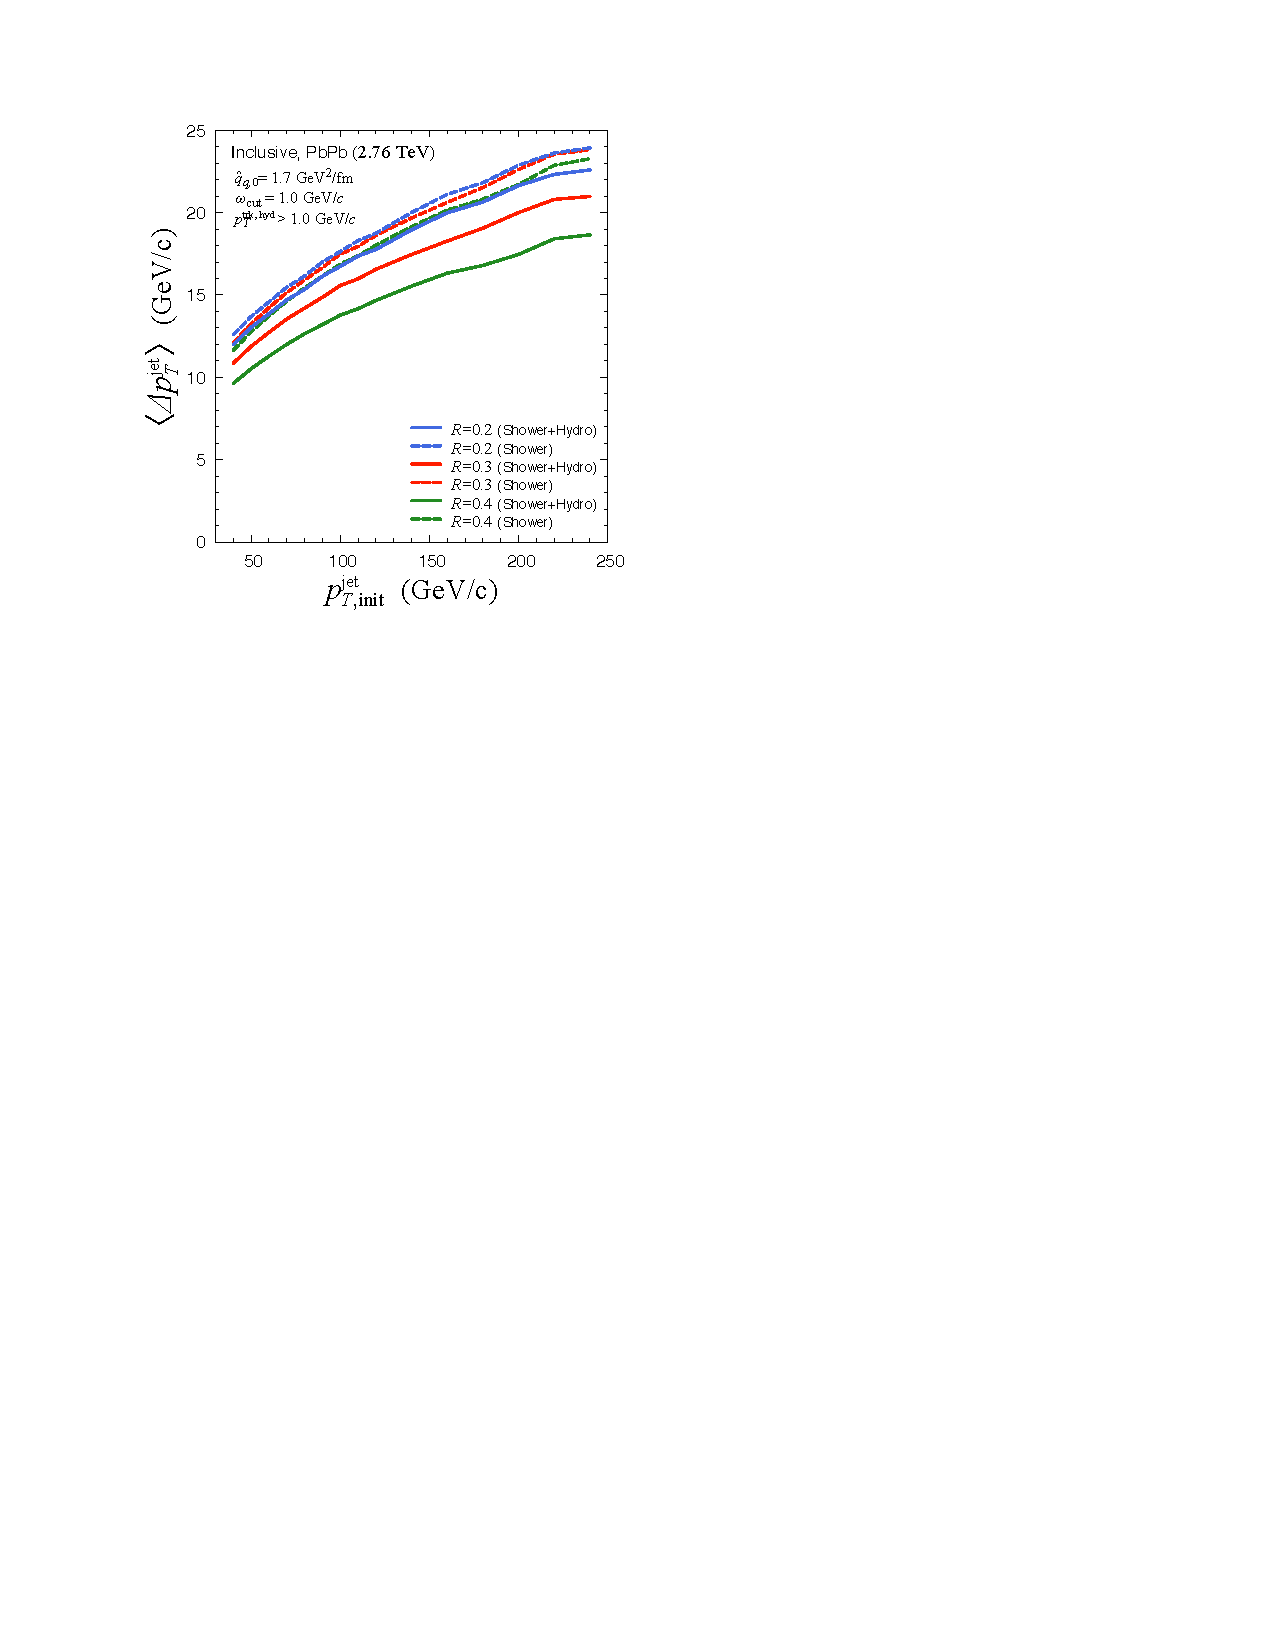
\includegraphics[ width=\textwidth]{figures/jetMeasurements/JF_energyLoss}
\caption{(Top) The energy lost by a jets of different radii as a function of their initial energy in central \pbpb\ collisions at \sqrtsnn = 2.76 TeV.
Figure from Ref.~\cite{Tachibana:2017syd}.}
\label{fig:jf_energyLoss}
  \end{minipage}
 \qquad  \qquad  \qquad
  \begin{minipage}[b]{0.43\textwidth}
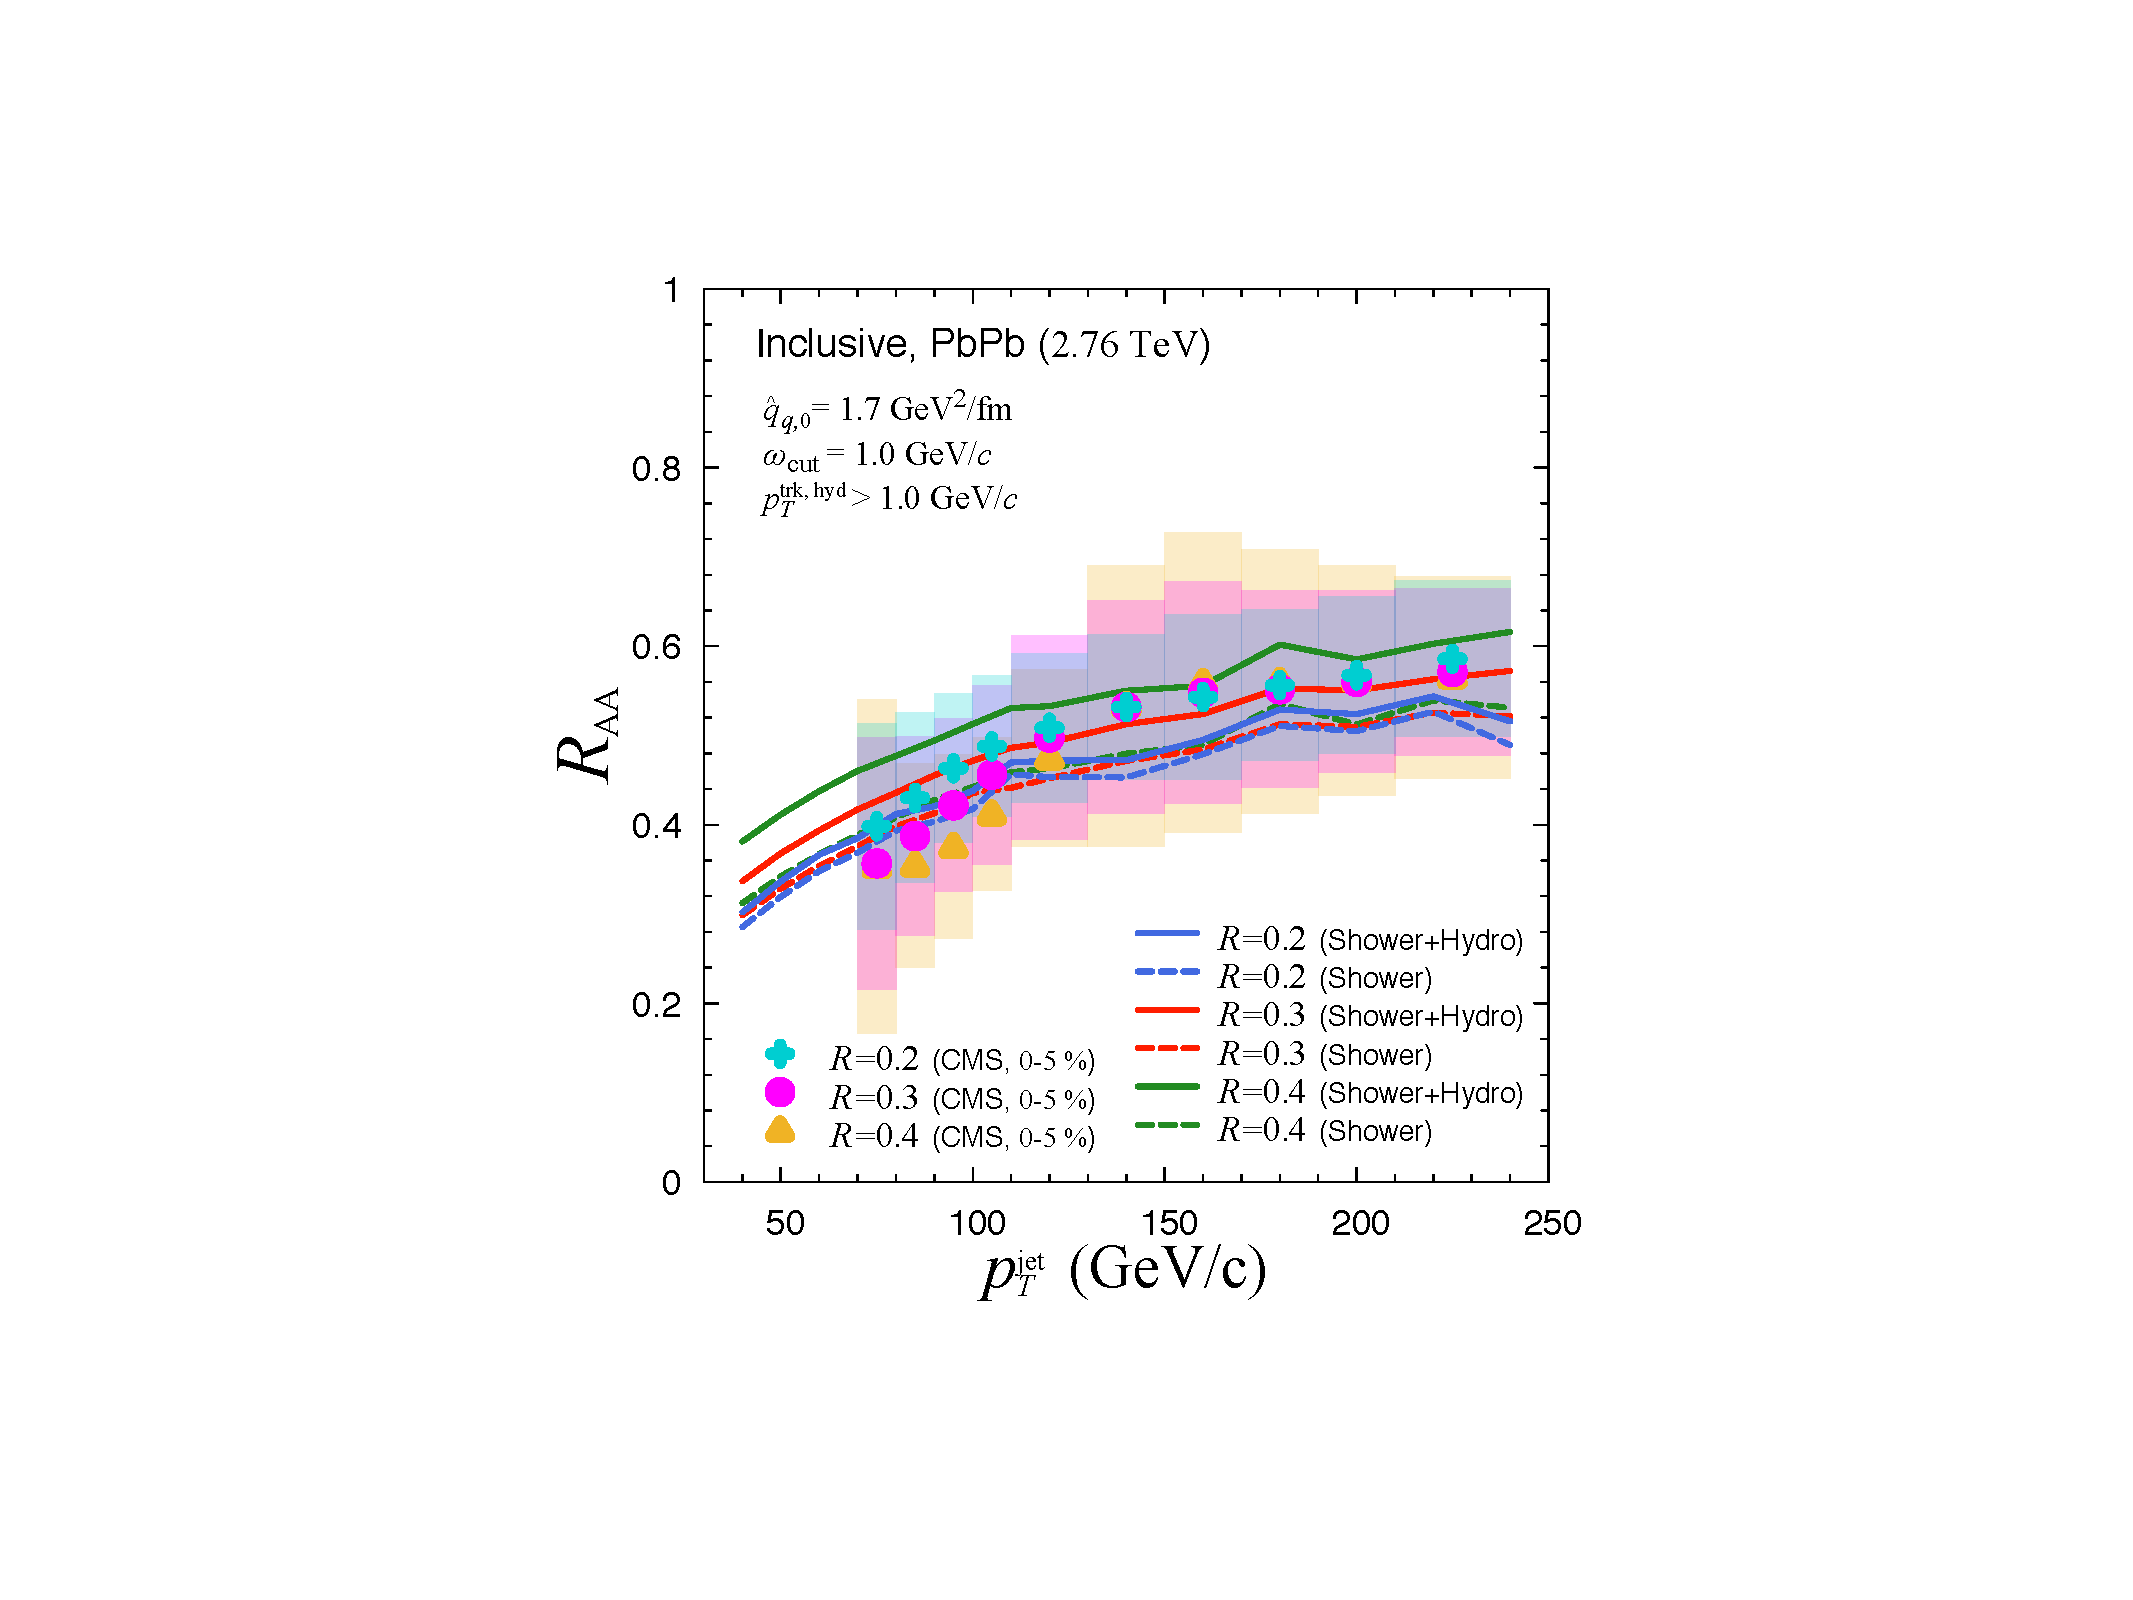
\includegraphics[width=\textwidth]{figures/jetMeasurements/JF_RAA}
\caption{The jet \RAA\ measured by CMS \cite{Khachatryan:2016jfl} and compared to the Jet-Fluid model with and without the hydro dynamic contribution.
Figure from Ref.~\cite{Tachibana:2017syd}.}
\label{fig:jf_raa}
  \end{minipage}
  \end{center}
\end{figure}



%\begin{figure}[htbp]
%\begin{center}
%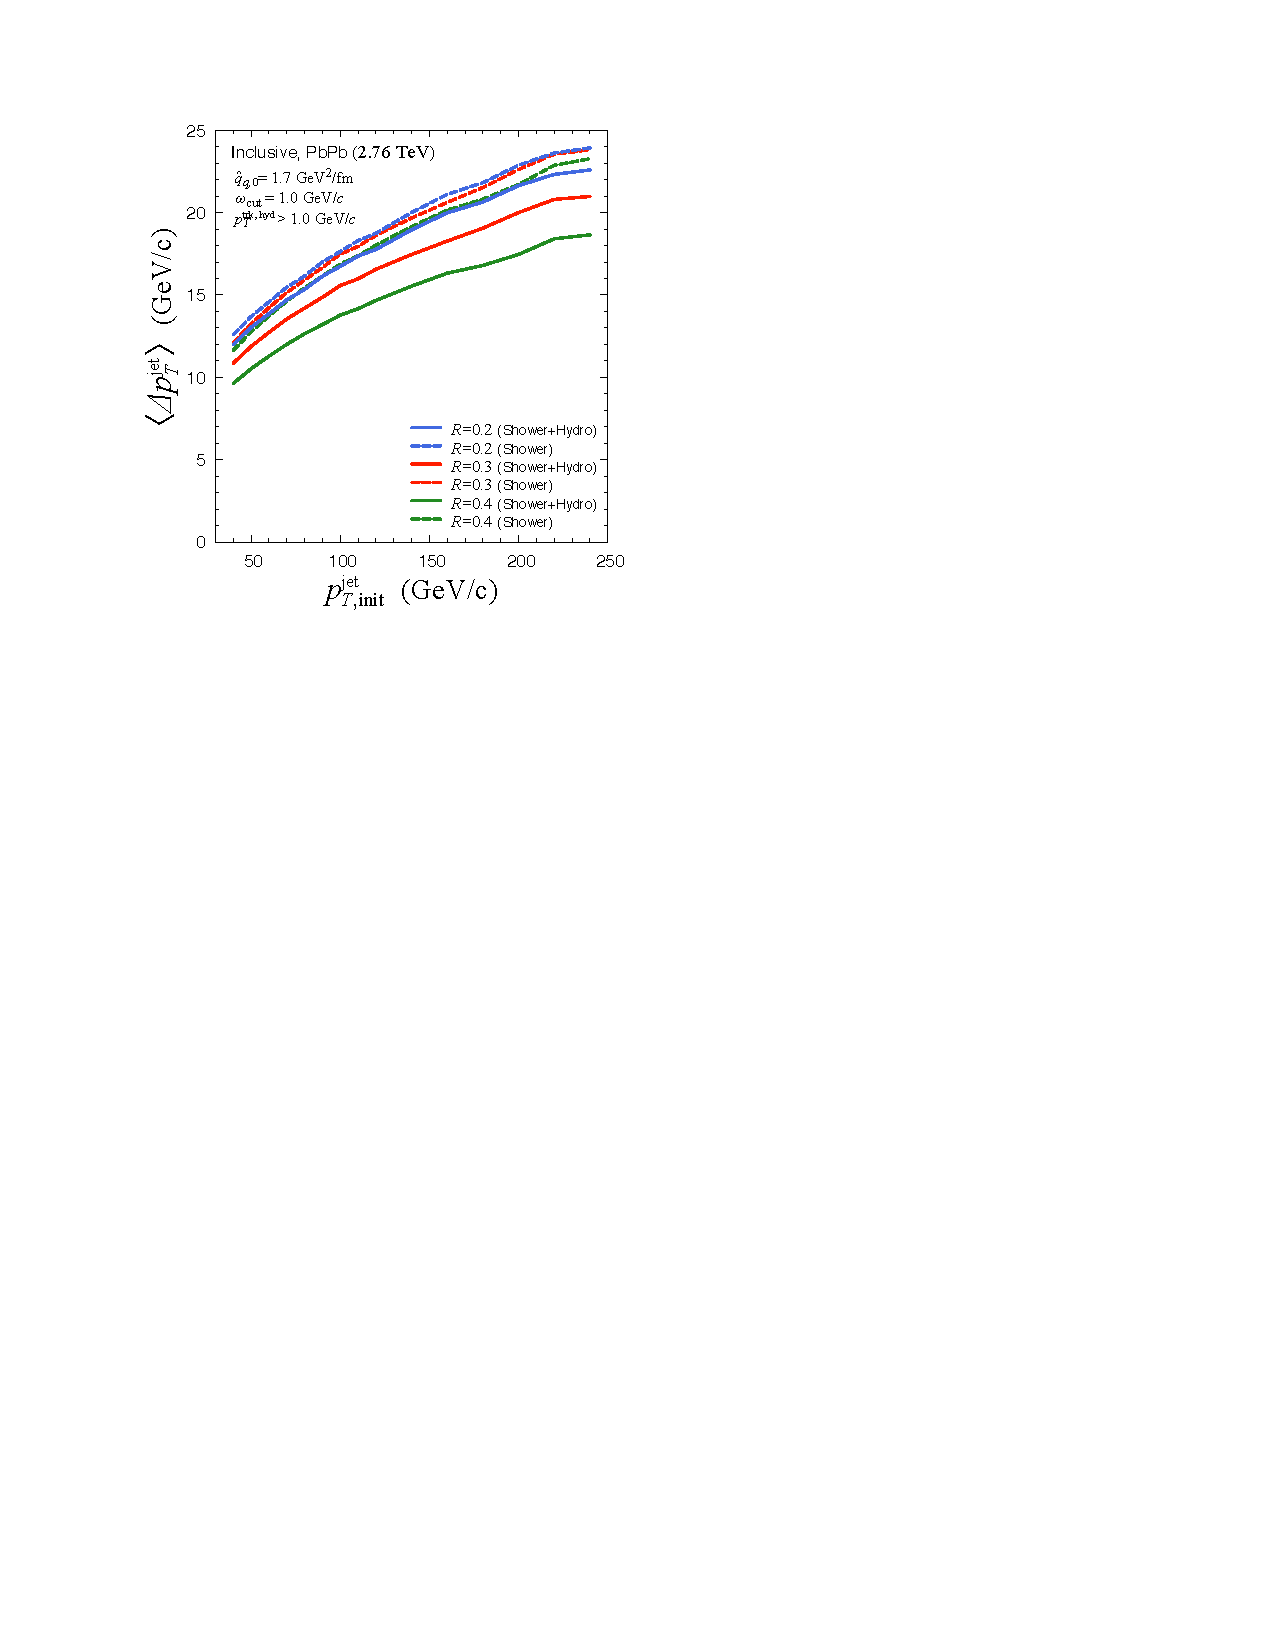
\includegraphics[width=0.45\textwidth]{figures/jetMeasurements/JF_energyLoss}
%\caption{(Top) The energy lost by a jets of different radii as a function of their initial energy in central \pbpb\ collisions at \sqrtsnn = 2.76 TeV.
%Figure taken from Ref.~\cite{Tachibana:2017syd}.}
%\label{fig:jf_energyLoss}
%\end{center}
%\end{figure}

The \RAA\ distributions constructed with this model and compared to data from CMS \cite{Khachatryan:2016jfl} are shown in Figure~\ref{fig:jf_raa}.
Including the hydrodynamic contribution decreases the energy loss, hence increasing the \RAA\ value and inducing a cone size dependence to the \RAA.

%\begin{figure}[htbp]
%\begin{center}
%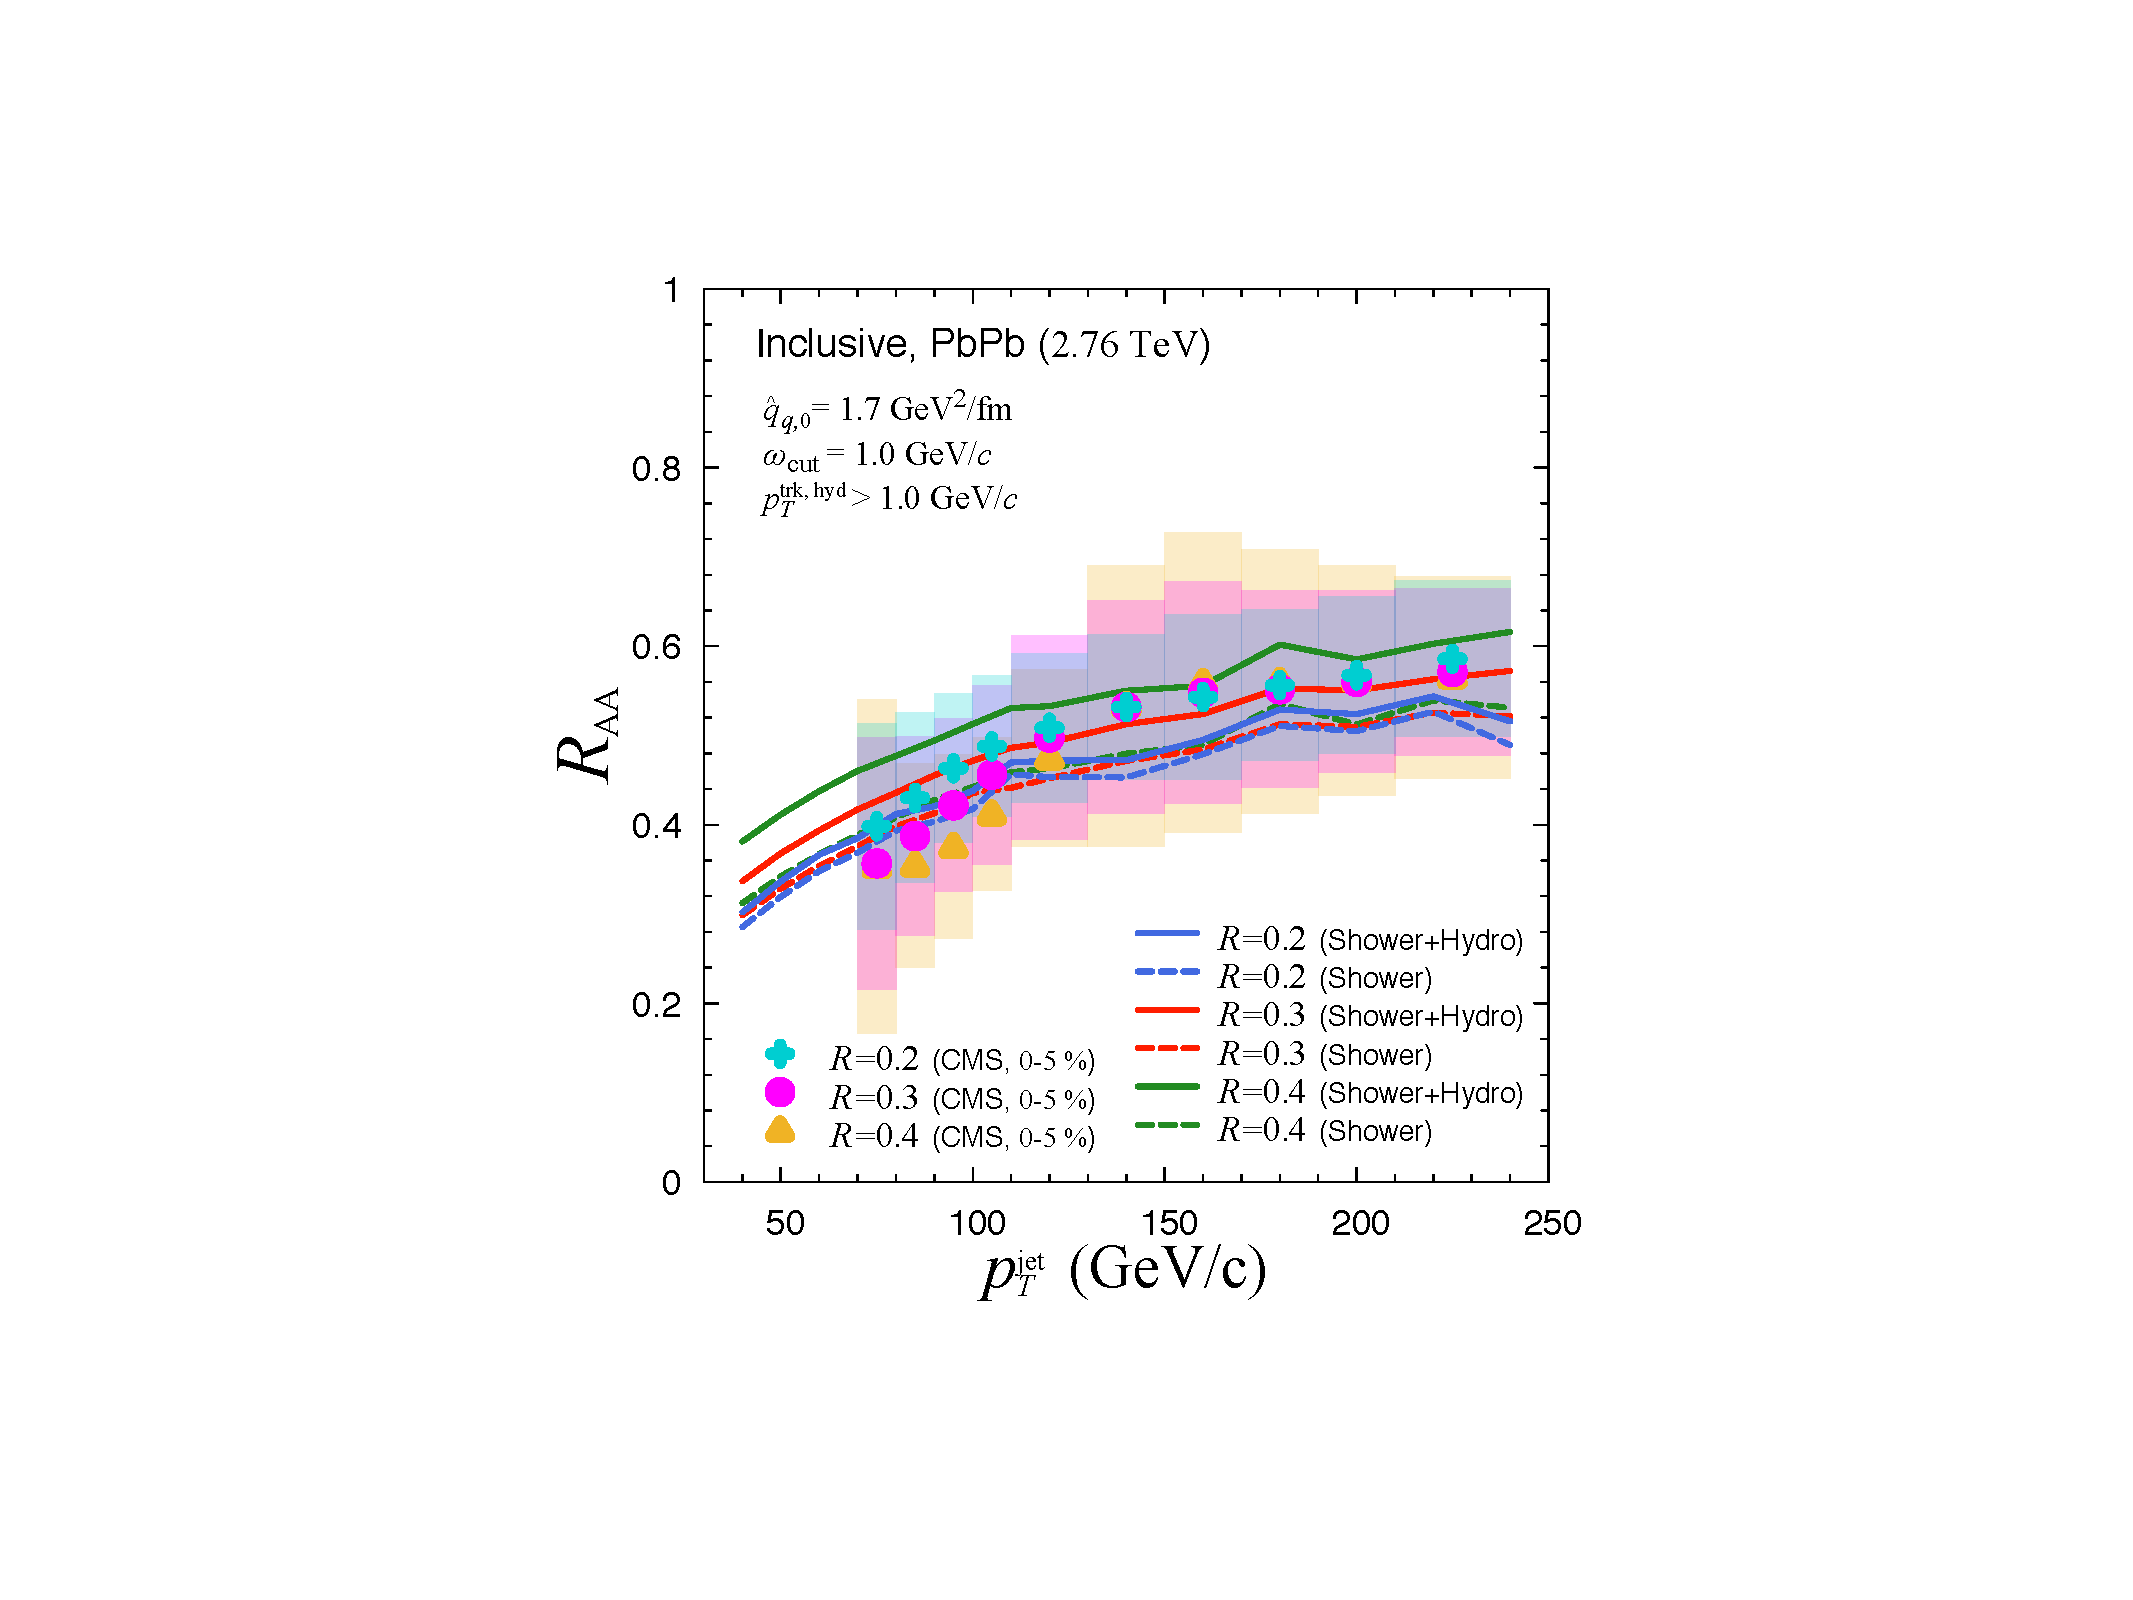
\includegraphics[width=0.45\textwidth]{figures/jetMeasurements/JF_RAA}
%\caption{The nuclear modification factor \RAA\ as a function of jet \pt\ as determined by the Jet-Fluid model and compared to the data measured by CMS \cite{Khachatryan:2016jfl}.
%The different colors represent different sized jets, with the dashed lines showing the modeled \RAA\ without the hydro-contribution.
%There is good agreement within the large uncertainties in the data.
%Figure taken from Ref.~\cite{Tachibana:2017syd}.}
%\label{fig:jf_raa}
%\end{center}
%\end{figure}

The internal structure of the jet can be described using the jet shape variable, defined as a per-jet quantity as:

\begin{align}
\rho_{\rm jet} = \frac{1}{\Njet} \sum_{\rm jet} \left[ \frac{1}{\ptjet} \frac{\sum_{\rm trk} \pttrk}{\delta r}  \right]
\end{align}
where the sum is over all jets and for all tracks around a jet in an annulus with mean radius $r$ from the jet axis.
The modification in the jet structure then can be defined as $R_{\rm AA}^\rho = \rho_{\rm AA} (r) / \rho_{\rm pp} (r) $.
%
%\begin{align}
%R_{\rm AA}^\rho = \dfrac{\rho_{\rm AA} (r) }{\rho_{\rm pp} (r) }
%\end{align}
A comparison of the jet shape variable $\rho$ and its modification $R_{\rm AA}^\rho$ to data measured by CMS is seen in Figure~\ref{fig:JF_jetShapemodel}.
The shower and hydro contributions are shown individually.
These indicate that the shower contribution to the jet shape variable is falls steeply as a function of distance from the jet axis while the hydro contribution is fairly constant at large distances.
This is because the energy loss from the shower is carried away by the jet induced flow to large angles.
The $R_{\rm AA}^\rho$ distribution further shows that the core is largely unmodified while the outer part of the jet is broadened.
The hydro-contribution mainly has an effect at larger distances from the jet axis.
This is consistent with the cone-size dependence seen in Figure~\ref{fig:jf_energyLoss}.

This model is particularly useful because it identifies both the effect of the medium on the jet, as well as the effect of the jet on the medium.

\begin{figure}
\begin{subfigure}{.45\textwidth}
  \centering
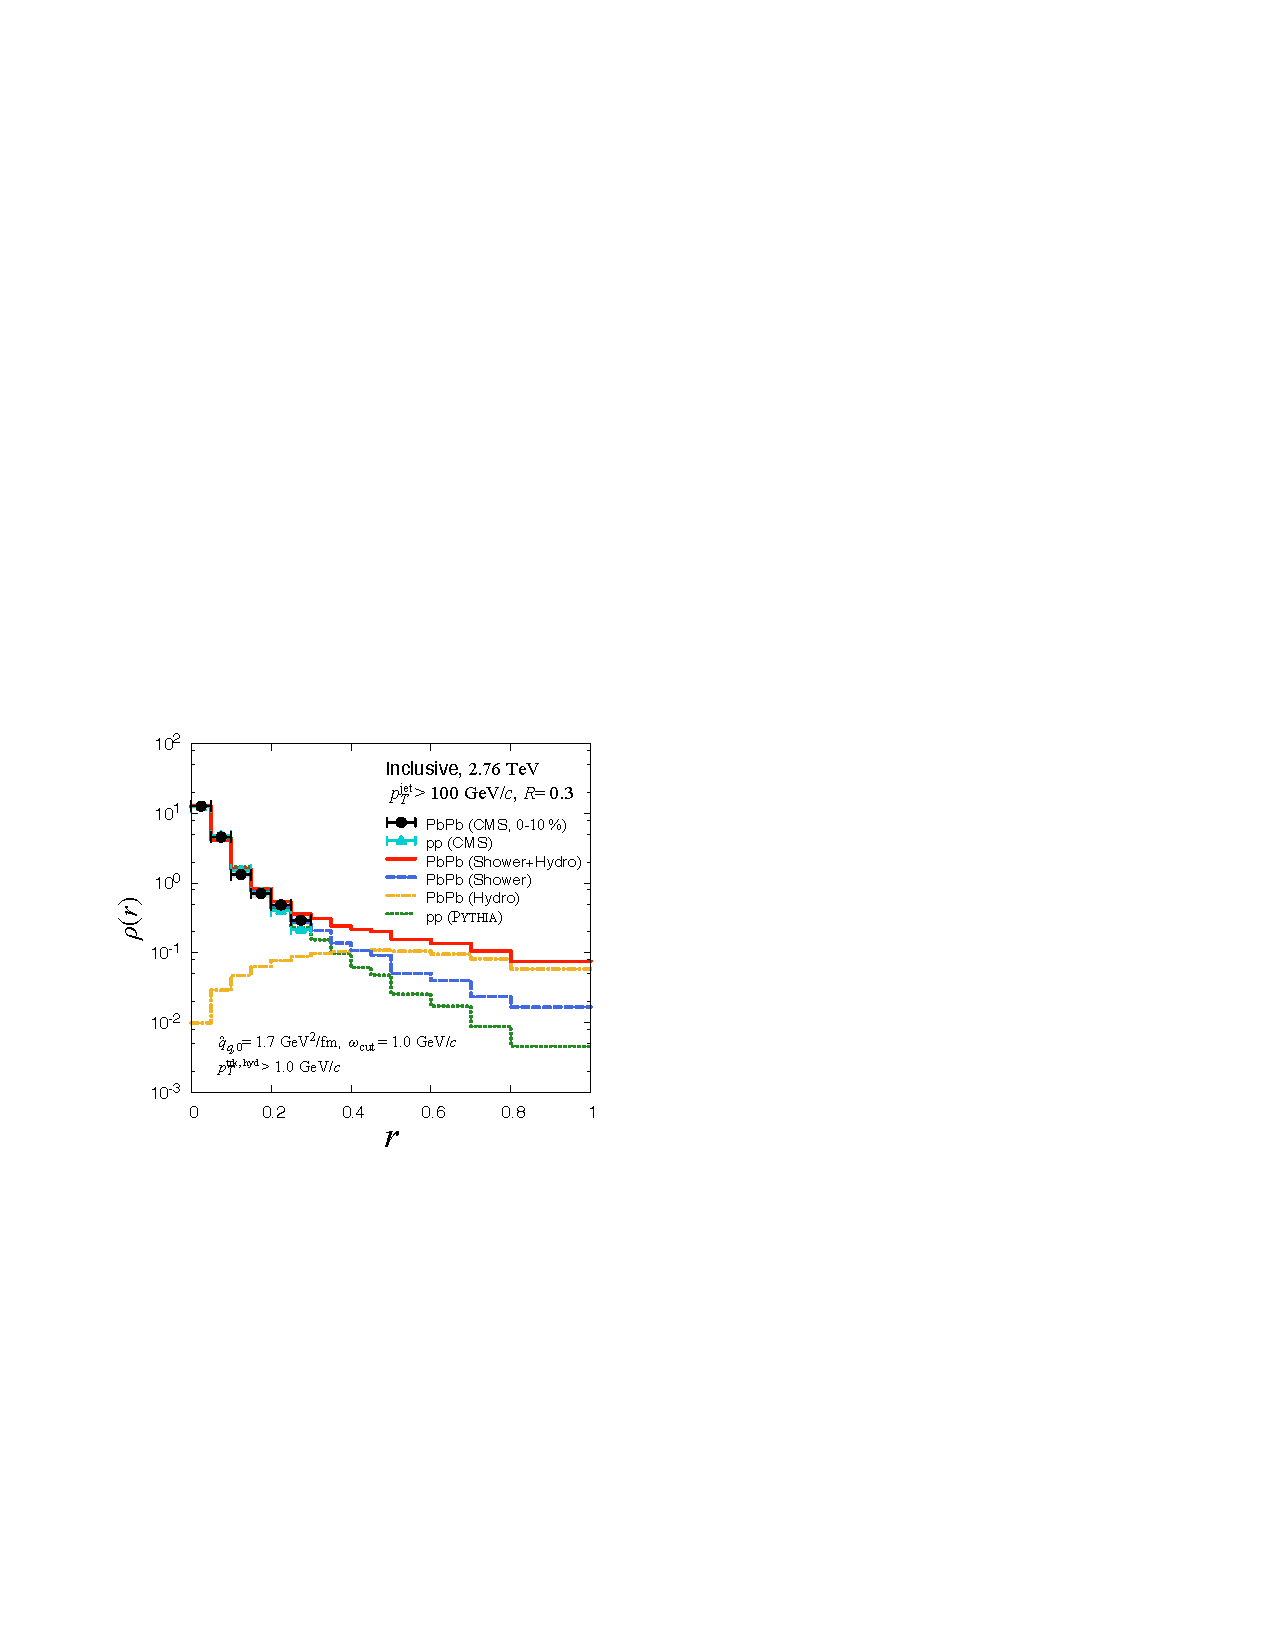
\includegraphics[width=0.95\textwidth]{figures/jetMeasurements/JF_jetShape}
\caption{The jet shape as measured by CMS for \pp\ and central \pbpb\ collisions \cite{Chatrchyan:2013kwa} compared to the Jet Fluid model.
The shower (blue) and hydro (orange) contributions to the jet shape are highlighted.}
\label{fig:jf_jetshape}
\end{subfigure} \qquad
\begin{subfigure}{.45\textwidth}
  \centering
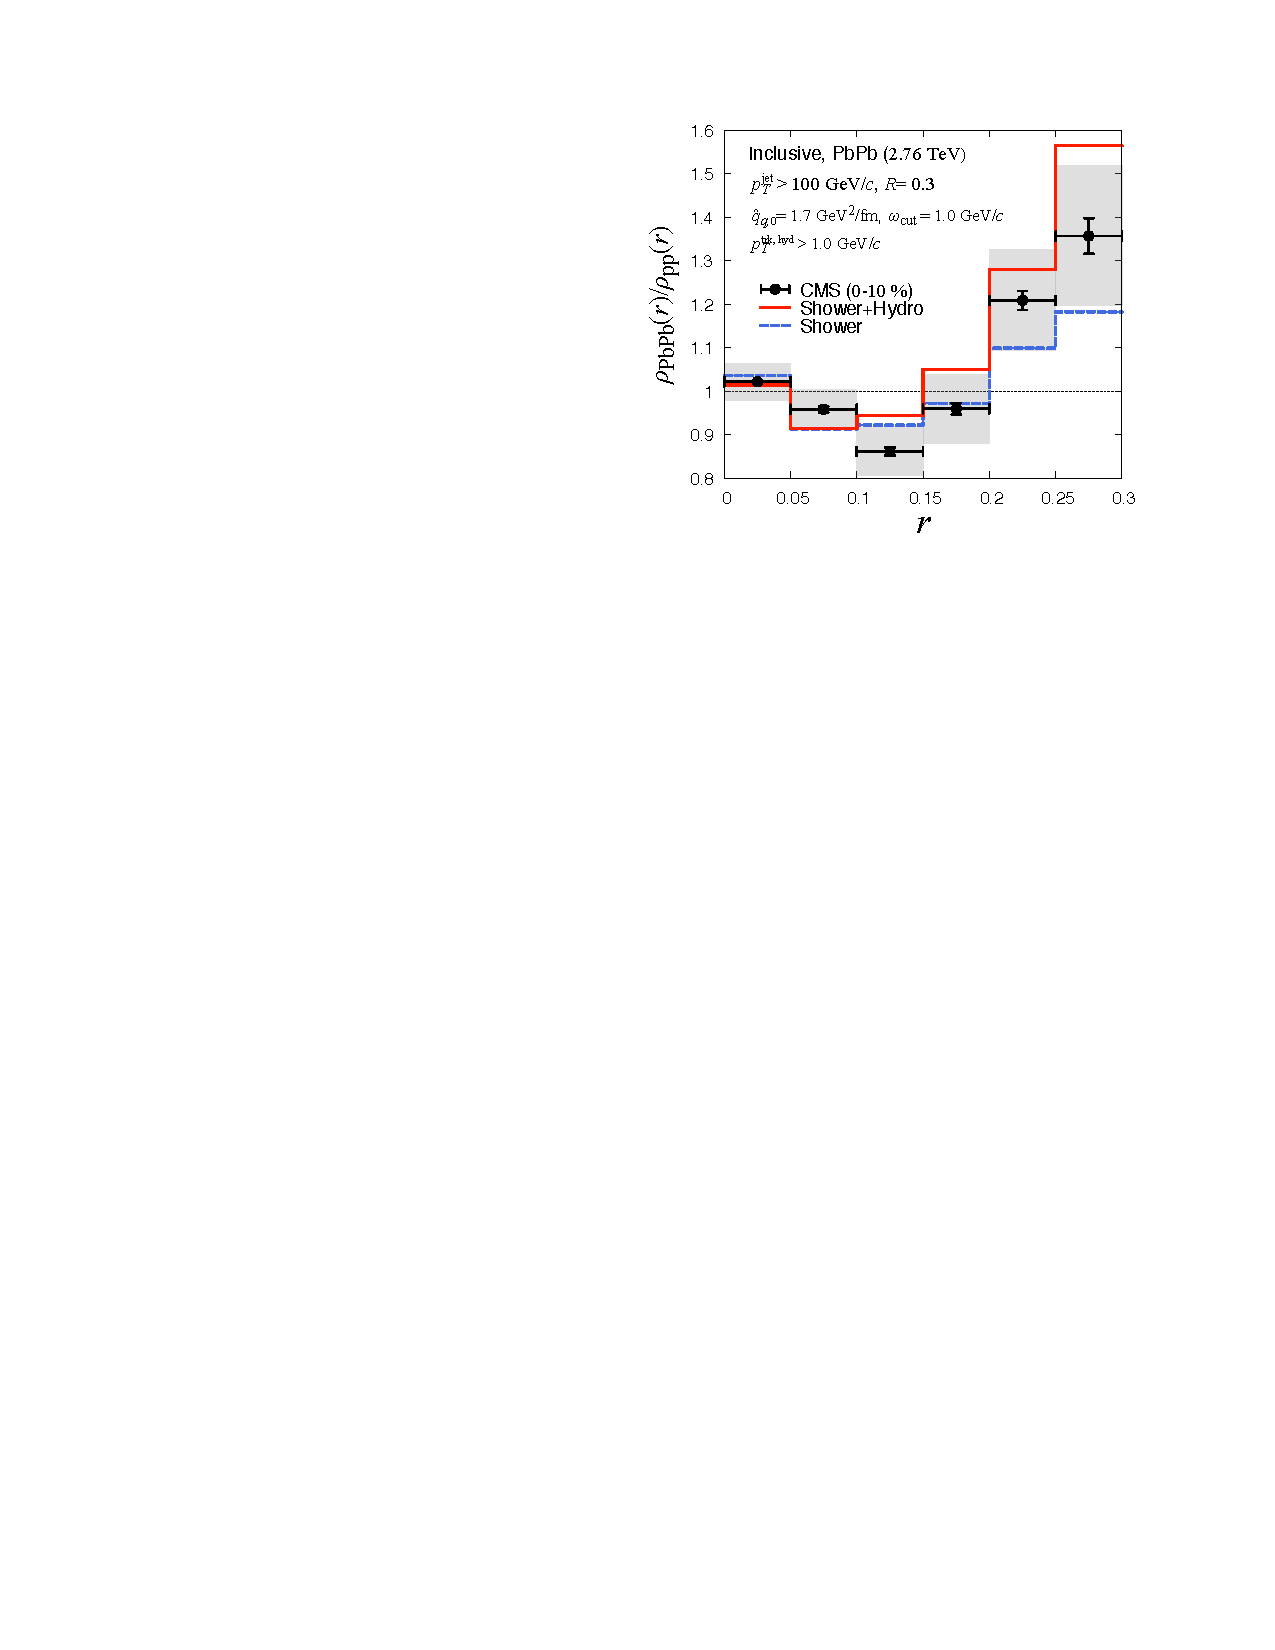
\includegraphics[width=0.95\textwidth]{figures/jetMeasurements/JF_jetShapeModification}
\caption{The modification of the jet shape between \pp\ and \pbpb\ as measured by CMS \cite{Chatrchyan:2013kwa} and compared to the Jet Fluid model.
The dashed line shows the modeled modification without the hydro-contribution.}
\label{fig:jf_jetshapemod}
\end{subfigure}
\caption{CMS data fit to calculations from the Jet Fluid model.
Figures from Ref.~\cite{Tachibana:2017syd}.}
\label{fig:JF_jetShapemodel}
\end{figure}



%\begin{align}
%\frac{d f_j}{dt} =& \left( \hat{e_j} \frac{\p}{\p \omega_j} + \frac{1}{4} \hat{q_j} \nabla_{\kT}^2\right) f_j  \\
%& + \sum_i \int d\omega_i d\kTsq_i \frac{d\widetilde{\Gamma}_{i\rightarrow j} (\omega_j, \kTsq_j | \omega_i, \kTsq_i)}{d\omega_j d\kTsq dt} f_i \\
%& - \sum_i \int d\omega_i d\kTsq_i \frac{d\widetilde{\Gamma}_{j\rightarrow i} (\omega_i, \kTsq_i | \omega_j, \kTsq_j)}{d\omega_j d\kTsq dt} f_i \\
%\end{align}
